\documentclass[13pt,a4paper]{extarticle}
\usepackage[utf8]{inputenc}
\usepackage[utf8]{vietnam} %Bien dich duoc tieng Viet
\usepackage{amsmath,amsfonts,amssymb} %Font toan
\usepackage{type1cm}
\usepackage{times}
\usepackage{graphicx}
\graphicspath{ {images04/} }
\usepackage{enumerate}
\usepackage{comment}
\usepackage{multicol}
\usepackage{multirow}
%\usepackage[unicode]{hyperref} %Tu dong tao bookmark
\usepackage[unicode, hidelinks=true]{hyperref}
\usepackage{indentfirst} %Thut vao dau dong o tat ca cac doan
\usepackage{listings} %Dinh dang code
\usepackage{color} %Mau sac
\usepackage[left=2.5cm,right=2.5cm,top=2.5cm,bottom=2.5cm]{geometry} %Canh lề trái - phải - trên - dưới cho tài liệu
\usepackage{longtable}
\renewcommand{\arraystretch}{1.3}

\begin{document}
\pagenumbering{gobble}
\title{\Large{\textbf{BÀI CHUẨN BỊ THỰC TẬP ĐIỆN CÔNG NGHIỆP}}\\\vspace{1cm}\textbf{Bài 4}\\\vspace{.5cm}\textbf{VẬN HÀNH ĐỘNG CƠ KĐB BA PHA VỚI CÁC KHÍ CỤ ĐIỆN VÀ BỘ KHỞI ĐỘNG MỀM}}
\date{Ngày 31 tháng 05 năm 2016}
%\date{\today}
\author{GVHD: Võ Minh Thiện \vspace{.6cm}\\  Nhóm SVTH: Nhóm 2 -- Tiểu nhóm 1: Thi Minh Nhựt}
\maketitle
\tableofcontents
\newpage
\pagenumbering{arabic}
\setcounter{page}{1}
\section{Chuẩn bị}
\begin{list}{--}{}
\item Mô hình vận hành động cơ bằng các khí cụ điện, bộ khởi động mềm.
\item Bộ thiết bị đo dòng, đo áp hiển thị kim.
\item Động cơ điện (loại 3 pha $380/660V$).
\end{list}
\section{Vận hành động cơ không đồng bộ ba pha bằng các khí cụ điện}
\subsection{Vận hành khởi động sao -- tam giác}
Thực hiện theo các bước sau:
\begin{list}{--}{}
\item \textit{Bước 1}: Lắp mạch động lực và mạch điều khiển theo sơ đồ hình ~\ref{Fig:1}. \textit{Nối đất thiết bị}.
\begin{figure}[!h]
\begin{center}
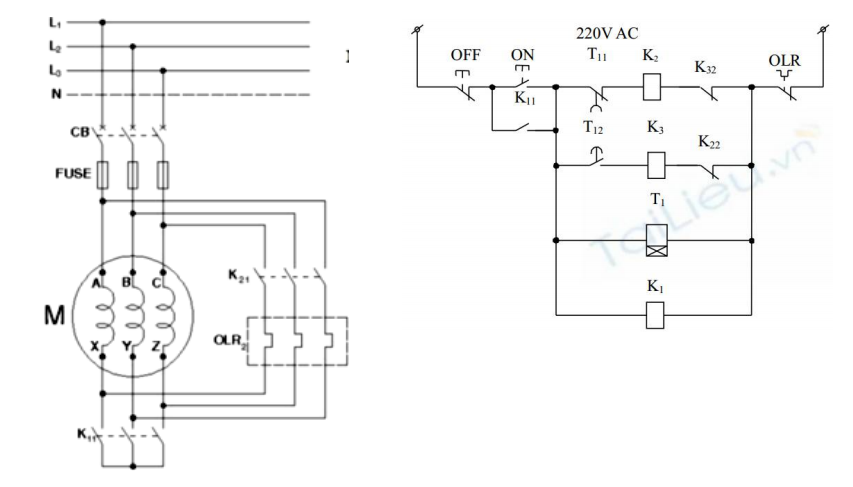
\includegraphics[scale=.6]{1}
\end{center}
\caption{Mạch động lực và mạch điều khiển khởi động sao -- tam giác}\label{Fig:1}
\end{figure}
\item \textit{Bước 2}: Nhờ GVHD kiểm tra, bật CB vận hành mạch điều khiển trước khi vận hành mạch động lực. 
\item \textit{Bước 3}: Đấu dây mạch động lực và nhấn nút ON.
\item \textit{Bước 4}: Điền các số liệu vào bảng:
\begin{center}
\begin{tabular}{|c|c|c|c|}\hline
\textit{Điện áp vận hành} & \textit{Dòng khởi động} & \textit{Dòng không tải} & \textit{Công suất không tải}\\ 
$V$ & $A$ & $A$ & $W$ \\ \hline
$U_{AB}= $&$I_A = $ & $I_A = $ & \\ \hline
$U_{BC}= $&$I_B = $ & $I_B = $ & \\ \hline
$U_{AC}= $&$I_C = $ & $I_C = $ & \\ \hline
\end{tabular}
\end{center}
\item \textit{Bước 5}: Nhấn nút $OFF$ để kết thúc vận hành và tắt nguồn CB.
\end{list}
\subsection{Động cơ không đồng bộ ba pha đảo chiều quay}
Thực hiện theo các bước:
\begin{list}{--}{}
\item \textit{Bước 1}: Lắp mạch động lực và mạch điều khiển theo sơ đồ hình ~\ref{Fig:2}. \textit{Nối đất thiết bị}.
\begin{figure}[!h]
\begin{center}
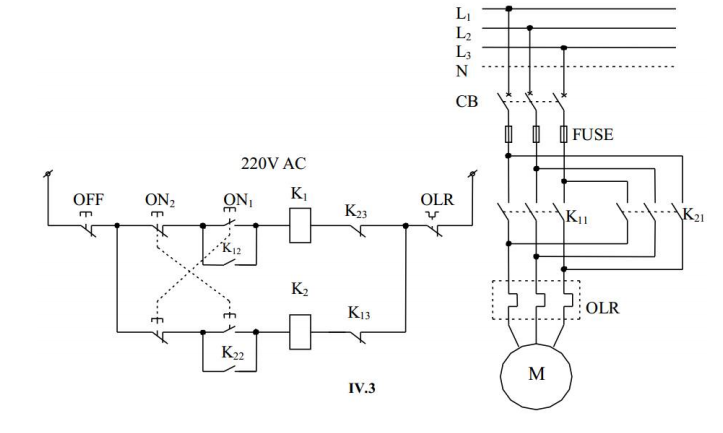
\includegraphics[scale=.6]{2}
\end{center}
\caption{Mạch động lực và mạch điều khiển đảo chiều quay động cơ}\label{Fig:2}
\end{figure}
\item \textit{Bước 2}: Nhờ GVHD kiểm tra, bật CB vận hành mạch điều khiển trước khi vận hành mạch động lực. 
\item \textit{Bước 3}: Đấu dây mạch động lực và nhấn nút ON.
\item \textit{Bước 4}: Điền các số liệu vào bảng:
\begin{center}
\begin{tabular}{|c|c|c|c|}\hline
\textit{Điện áp vận hành} & \textit{Dòng khởi động} & \textit{Dòng không tải} & \textit{Công suất không tải}\\ 
$V$ & $A$ & $A$ & $W$ \\ \hline
$U_{AB}= $&$I_A = $ & $I_A = $ & \\ \hline
$U_{BC}= $&$I_B = $ & $I_B = $ & \\ \hline
$U_{AC}= $&$I_C = $ & $I_C = $ & \\ \hline
\end{tabular}
\end{center}
\item \textit{Bước 5}: Nhấn nút $OFF$ để kết thúc vận hành và tắt nguồn CB.
\end{list}
\subsection{Vận hành động cơ không đồng bộ 3 pha chạy 2 cấp tốc độ}
\begin{list}{--}{}
\item \textit{Bước 1}: Lắp mạch động lực và mạch điều khiển theo sơ đồ hình ~\ref{Fig:3}. \textit{Nối đất thiết bị}.
\begin{figure}[!h]
\begin{center}
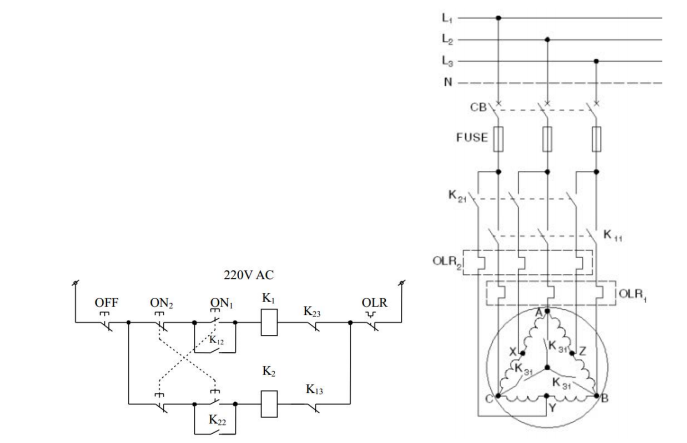
\includegraphics[scale=.6]{3}
\end{center}
\caption{Mạch động lực và mạch điều khiển chạy 2 cấp tốc độ}\label{Fig:3}
\end{figure}
\item \textit{Bước 2}: Nhờ GVHD kiểm tra, bật CB vận hành mạch điều khiển trước khi vận hành mạch động lực. 
\item \textit{Bước 3}: Đấu dây mạch động lực và nhấn nút ON.
\item \textit{Bước 4}: Điền các số liệu vào bảng:
\begin{center}
\begin{tabular}{|c|c|c|c|}\hline
\textit{Điện áp vận hành} & \textit{Dòng khởi động} & \textit{Dòng không tải} & \textit{Công suất không tải}\\ 
$V$ & $A$ & $A$ & $W$ \\ \hline
$U_{AB}= $&$I_A = $ & $I_A = $ & \\ \hline
$U_{BC}= $&$I_B = $ & $I_B = $ & \\ \hline
$U_{AC}= $&$I_C = $ & $I_C = $ & \\ \hline
\end{tabular}
\end{center}
\item \textit{Bước 5}: Nhấn nút $OFF$ để kết thúc vận hành và tắt nguồn CB.
\end{list}
\subsection{Vận hành động cơ không đồng bộ 3 pha bằng bộ khởi động mềm}
\begin{list}{--}{}
\item \textit{Bước 1}: Mô hình khởi động mềm như hình ~\ref{Fig:4}.
\begin{figure}[!h]
\begin{center}
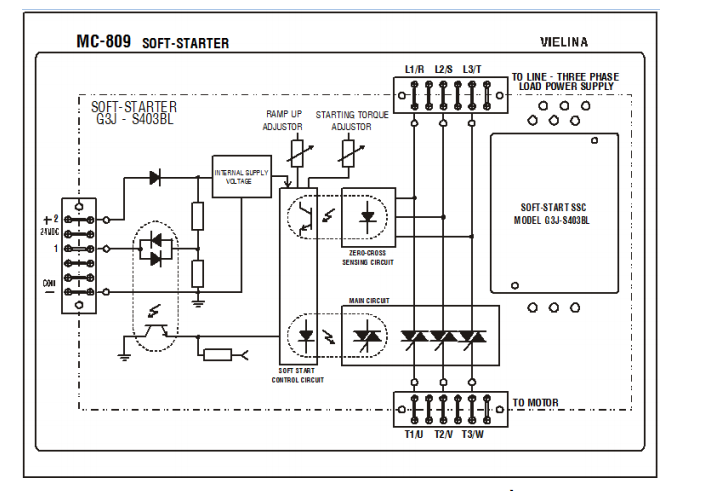
\includegraphics[scale=.6]{4}
\end{center}
\caption{Mô hình khởi động mềm}\label{Fig:4}
\end{figure}
\item \textit{Bước 2}: Lắp mạch động lực và mạch điều khiển theo sơ đồ hình ~\ref{Fig:5}. \textit{Nối đất thiết bị}.
\begin{figure}[!h]
\begin{center}
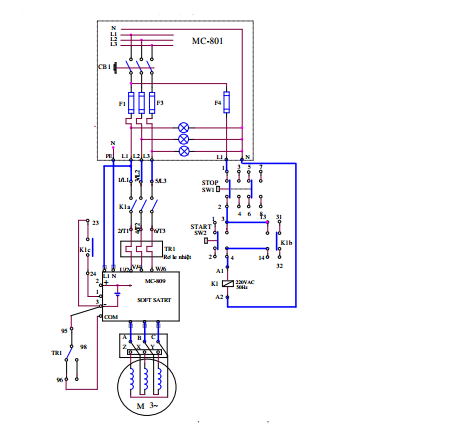
\includegraphics[scale=1.5]{5}
\end{center}
\caption{Mạch động lực và mạch điều khiển cho khởi động mềm}\label{Fig:5}
\end{figure}
\item \textit{Bước 3}: Nhờ GVHD kiểm tra, bật CB vận hành mạch điều khiển trước khi vận hành mạch động lực. 
\item \textit{Bước 4}: Đấu dây mạch động lực và nhấn nút START. Quan sát hiện tượng.
\item \textit{Bước 5}: Điền các số liệu vào bảng:
\begin{center}
\begin{tabular}{|c|c|c|c|}\hline
\textit{Điện áp vận hành} & \textit{Dòng khởi động} & \textit{Dòng không tải} & \textit{Công suất không tải}\\ 
$V$ & $A$ & $A$ & $W$ \\ \hline
$U_{AB}= $&$I_A = $ & $I_A = $ & \\ \hline
$U_{BC}= $&$I_B = $ & $I_B = $ & \\ \hline
$U_{AC}= $&$I_C = $ & $I_C = $ & \\ \hline
\end{tabular}
\end{center}
\item \textit{Bước 6}: Nhấn nút $OFF$ để kết thúc vận hành và tắt nguồn CB.
\end{list}
\end{document}